\documentclass[11pt]{article}
\usepackage[margin=1in]{geometry}
\usepackage{amsmath,amssymb}
\usepackage{listings}
\usepackage{xcolor}
\usepackage{hyperref}
\usepackage{tikz}
\usetikzlibrary{positioning, arrows.meta}

\lstset{
  basicstyle=\ttfamily\small,
  keywordstyle=\color{black}\bfseries,
  commentstyle=\color{gray},
  breaklines=true,
  frame=single,
  framerule=0.4pt,
  xleftmargin=1em,
  framexleftmargin=0.5em,
  columns=fullflexible,
  keepspaces=true,
  aboveskip=1em,
  belowskip=1em,
  escapeinside={(*@}{@*)},
}

\definecolor{accentgray}{RGB}{100,100,100}
\newcommand{\deferred}[1]{\textcolor{accentgray}{\textit{// deferred: #1}}}

\title{FEN Schema for C-SQD\\[0.4em]
\large Facts, Episodes, and Narratives as Epistemic Audit Infrastructure}
\author{Marcus Thomas}
\date{June 2026}

\begin{document}
\maketitle
\tableofcontents
\newpage

% ─────────────────────────────────────────────
\section{Overview}
% ─────────────────────────────────────────────

This document specifies the internal data schema for C-SQD, adapted from the
Facts, Episodes, and Narratives (FEN) architecture originally developed for
Phoros. FEN organizes data into three ontological layers: atomic events
(\textbf{Facts}), problem-centric groupings (\textbf{Episodes}), and authored
interpretations (\textbf{Narratives}). These layers map onto C-SQD's epistemic
auditing architecture with structural fidelity.

The mapping is as follows:

\begin{center}
\renewcommand{\arraystretch}{1.4}
\begin{tabular}{l l l}
\textbf{FEN Primitive} & \textbf{C-SQD Realization} & \textbf{Ontological Status} \\
\hline
Fact      & \texttt{Fact} (commission, element review, solicitation, \ldots) & Atomic epistemic act \\
Episode   & \texttt{AuditEpisode}       & Coherent audit question over time \\
Narrative & \texttt{SynthesisReview}    & Authored integrative interpretation \\
\end{tabular}
\end{center}

The \textbf{audit subject} --- a paper, model, clinical trial protocol, dataset,
benchmark, or other artifact under evaluation --- is not an ontological
primitive. It is the \texttt{subject\_id} referent on every \texttt{Fact}: the
thing the facts are \emph{about}. This is analogous to the patient in clinical
FEN. The same audit subject may be referenced by multiple independent
\texttt{AuditEpisode}s commissioned by different sponsors at different times.

C-SQD extends FEN in two directions. First, \texttt{DomainInstantiation} is a
first-class configuration layer above episodes, capturing the platform's
multi-domain generality: academic publishing, clinical trial review, AI
auditing, policy review, and others. Second, the \textbf{evaluation tuple}
$E(A \mid R, T_\text{eval}) \to (N, M, S, L, U)$ is a derived view computed
over accumulated \texttt{EpisodeMembership} records, recomputable for any
reviewer community and reference time. It is not stored state.

The schema is defined as Rust types. Storage is abstracted.

\subsection{Entity Layers}

\begin{center}
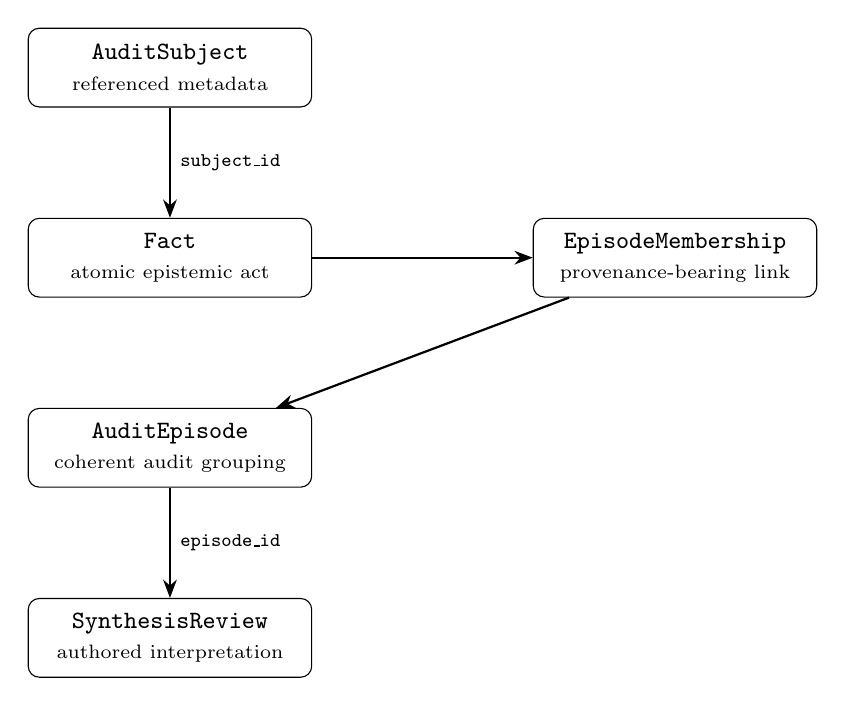
\begin{tikzpicture}[
  box/.style={draw, rounded corners, minimum width=3.6cm, minimum height=1cm,
              align=center, font=\small},
  edge/.style={-{Stealth}, thick},
  node distance=1.4cm
]
  \node[box] (subject) {\texttt{AuditSubject}\\{\scriptsize referenced metadata}};
  \node[box, below=of subject] (fact) {\texttt{Fact}\\{\scriptsize atomic epistemic act}};
  \node[box, below=of fact] (episode) {\texttt{AuditEpisode}\\{\scriptsize coherent audit grouping}};
  \node[box, below=of episode] (narrative) {\texttt{SynthesisReview}\\{\scriptsize authored interpretation}};

  \node[box, right=2.8cm of fact] (membership) {\texttt{EpisodeMembership}\\{\scriptsize provenance-bearing link}};

  \draw[edge] (subject) -- node[right, font=\scriptsize]{\texttt{subject\_id}} (fact);
  \draw[edge] (fact) -- (membership);
  \draw[edge] (membership) -- (episode);
  \draw[edge] (episode) -- node[right, font=\scriptsize]{\texttt{episode\_id}} (narrative);
\end{tikzpicture}
\end{center}

% ─────────────────────────────────────────────
\section{Domain Instantiation}
% ─────────────────────────────────────────────

C-SQD may be instantiated in multiple domains. Each instantiation defines its
own CWE taxonomy, evaluation tuple configuration, and optional phase parameters.
\texttt{DomainInstantiation} is a first-class entity that owns this
configuration. Every downstream entity --- \texttt{AuditSubject}, \texttt{Fact},
\texttt{AuditEpisode} --- carries a \texttt{domain\_instantiation\_id} anchoring
it to its instantiation.

\begin{lstlisting}
struct DomainInstantiationId(Uuid);

struct DomainInstantiation {
    id:           DomainInstantiationId,
    domain_type:  DomainType,
    config:       DomainConfig,
    cwe:          CWETaxonomy,
    created_at:   Timestamp,
    governed_by:  Principal,
}

enum DomainType {
    AcademicPublishing,
    ClinicalTrialReview,
    AIAuditing,
    PolicyReview,
    Custom(String),
}
\end{lstlisting}

Multiple instantiations of the same \texttt{DomainType} are permitted. A
sponsored NIH review program and an independent conference partnership are both
\texttt{AcademicPublishing} instantiations with different configurations.

\subsection{Domain Configuration}

\begin{lstlisting}
struct DomainConfig {
    eval_tuple_config:    EvalTupleConfig,
    audit_subject_types:  Vec<AuditSubjectType>,
    phase_config:         Option<PhaseConfig>,
}
\end{lstlisting}

\texttt{PhaseConfig} is optional. Commissioned audits do not require the
three-phase public review structure; it is available for domain instantiations
that need it.

\begin{lstlisting}
struct PhaseConfig {
    public_review_duration:           Option<Duration>,
    response_rounds_permitted:        u32,
    synthesis_significance_threshold: f64,
    anonymity_rules:                  AnonymityConfig,
}
\end{lstlisting}

\subsection{The CWE Taxonomy}

The Common Weakness Enumeration (CWE) is an extensible node tree of evaluation
criteria. It is not a closed enum. Each node carries provenance indicating
whether it belongs to the base taxonomy or a community extension.

\begin{lstlisting}
struct CWENodeId(Uuid);

struct CWENode {
    id:                      CWENodeId,
    domain_instantiation_id: DomainInstantiationId,
    parent:                  Option<CWENodeId>,
    label:                   String,
    description:             String,
    source:                  CWESource,
}

enum CWESource {
    BaseTaxonomy,
    CommunityExtension { community_id: CommunityId }, (*@\deferred{post-MVP}@*)
}

// A CWECriterionId carries its domain context implicitly.
struct CWECriterionId {
    domain:   DomainInstantiationId,
    node_id:  CWENodeId,
}
\end{lstlisting}

% ─────────────────────────────────────────────
\section{Audit Subject}
% ─────────────────────────────────────────────

An \texttt{AuditSubject} is the artifact under evaluation: a research manuscript,
preprint, dataset, code repository, clinical trial protocol, AI model evaluation,
benchmark, policy document, grant proposal, or technical report. It is
\emph{not} an ontological primitive in the FEN sense. It is the referent of
\texttt{subject\_id} on every \texttt{Fact} --- the thing the facts are about.
The design rationale is discussed in Section~\ref{sec:subject-rationale}.

\begin{lstlisting}
struct AuditSubjectId(Uuid);

struct AuditSubject {
    id:                      AuditSubjectId,
    domain_instantiation_id: DomainInstantiationId,
    subject_type:            AuditSubjectType,
    title:                   Option<String>,
    external_refs:           Vec<ExternalRef>,
    registered_by:           Principal,
    registered_at:           Timestamp,
}

enum AuditSubjectType {
    ResearchManuscript,
    Preprint,
    Dataset,
    CodeRepository,
    ClinicalTrialProtocol,
    AIModelEvaluation,
    Benchmark,
    PolicyDocument,
    GrantProposal,
    TechnicalReport,
    Other(String),
}
\end{lstlisting}

An \texttt{AuditSubject} may be registered by a sponsor, an admin, or an
importer. It does not need to have been submitted by its author. The same
subject may be referenced by multiple independent \texttt{AuditEpisode}s.

% ─────────────────────────────────────────────
\section{Users and Organizations}
% ─────────────────────────────────────────────

Every platform participant is a \texttt{User}. Reviewer and submitter are roles
that context supplies, not distinct types. An \texttt{ElementReview} fact records
who reviewed; an \texttt{AuditCommission} fact records who sponsored. A user who
has completed reviewer onboarding carries a \texttt{ReviewerProfile}.

\begin{lstlisting}
struct UserId(Uuid);

struct User {
    id:               UserId,
    display_name:     String,
    email:            String,
    created_at:       Timestamp,
    status:           UserStatus,
    reviewer_profile: Option<ReviewerProfile>,
}

enum UserStatus {
    Active,
    Suspended { reason: String, until: Option<Timestamp> },
    Deactivated,
}
\end{lstlisting}

\texttt{Organization} is a first-class entity representing institutional
sponsors: biotechnology companies, venture capital firms, foundations,
universities, journals, and regulators.

\begin{lstlisting}
struct OrganizationId(Uuid);

struct Organization {
    id:         OrganizationId,
    name:       String,
    org_type:   OrganizationType,
    created_at: Timestamp,
}

enum OrganizationType {
    Biotech,
    VentureCapital,
    Foundation,
    University,
    Journal,
    Regulator,
    Other(String),
}
\end{lstlisting}

\texttt{Principal} is the reference type used in provenance and authorship
contexts. It identifies who asserted or performed something without carrying
the full entity record.

\begin{lstlisting}
enum Principal {
    User(UserId),
    Organization(OrganizationId),
    Platform,
    AiAssisted { tool_id: String, supervised_by: Option<UserId> },
}
\end{lstlisting}

\subsection{Reviewer Profile}

\texttt{ReviewerProfile} is a top-level entity keyed by \texttt{UserId},
fetched independently when reviewer-specific context is needed.

\begin{lstlisting}
struct ReviewerProfile {
    user_id:           UserId,
    status:            ReviewerStatus,
    tags:              Vec<ReviewerTag>,
    domain_extensions: Vec<ReviewerDomainExtension>,
}

enum ReviewerStatus {
    GracePeriod,
    Active,
    Suspended,
}

struct ReviewerTag {
    id:       TagId,
    label:    String,
    scope:    TagScope,
    verified: bool,
}

enum TagScope {
    Global,
    Domain(DomainInstantiationId),
}

struct ReviewerDomainExtension {
    domain_instantiation_id: DomainInstantiationId,
    data: serde_json::Value, // domain-specific fields
}
\end{lstlisting}

% ─────────────────────────────────────────────
\section{Facts}
% ─────────────────────────────────────────────

A \texttt{Fact} is the atomic unit of the C-SQD schema. It represents a single
epistemic or administrative act grounded in provenance: a sponsored audit
commission, a focused element review, a solicitation issued to a reviewer, a
solicitation lifecycle event, or a submitter response. Facts are time-indexed,
provenance-rich, and immutable. They are not updated; if a Fact is wrong or
superseded, its \texttt{status} changes and a new Fact may be created.

\begin{lstlisting}
struct FactId(Uuid);

struct Fact {
    id:                      FactId,
    subject_id:              AuditSubjectId,
    domain_instantiation_id: DomainInstantiationId,
    occurred_at:             Timestamp,
    payload:                 FactPayload,
    status:                  FactStatus,
    provenance:              Provenance,
    external_refs:           Vec<ExternalRef>,
}
\end{lstlisting}

\subsection{FactPayload}

\texttt{FactPayload} is a sum type carrying the type-specific data for each
fact variant. The set of variants is closed and controlled by C-SQD. This
design gives exhaustive pattern matching, value semantics, and no heap
allocation. The rationale for using an enum rather than trait objects is
discussed in Section~\ref{sec:enum-rationale}.

\begin{lstlisting}
enum FactPayload {
    AuditCommission {
        commissioned_by: Principal,
        scope:           Vec<CWECriterionId>,
        funding:         Money,
        deadline:        Option<Timestamp>,
        confidential:    bool,
    },
    ElementReview {
        cwe_criterion:   CWECriterionId,
        submitted_by:    UserId,
        solicitation:    Option<FactId>,   // ref to ERSolicitation fact
        finding:         Finding,
        severity:        Option<FindingSeverity>,
        confidence:      Option<ConfidenceLevel>,
        limitations:     Option<String>,
        recommendations: Option<String>,
        content:         String,
        featured:        bool,
    },
    ERSolicitation {
        issued_to:       UserId,
        cwe_criterion:   CWECriterionId,
        commission:      FactId,           // ref to AuditCommission fact
        payment_scheme:  PaymentScheme,
    },
    SolicitationEvent {
        solicitation:    FactId,           // ref to ERSolicitation fact
        event_type:      SolicitationEventType,
        principal:       Principal,
        note:            Option<String>,
    },
    SubmitterResponse {
        responding_to:   Vec<FactId>,
        response_type:   ResponseType,
        content:         String,
        revision_ref:    Option<AuditSubjectId>,
    },
    EpisodeParticipation {
        episode:         AuditEpisodeId,
        participant:     UserId,
        action:          ParticipationAction,   // Start | Join
        note:            Option<String>,
    },
    FeaturePetition {
        element_review:  FactId,                // ref to ElementReview fact
        petitioner:      UserId,
        rationale:       String,
    },
    CWEPetition {
        kind:            CWEPetitionKind,       // NewElement | Applicability
        cwe_node:        Option<CWENodeId>,
        proposed_label:  Option<String>,
        petitioner:      UserId,
        rationale:       String,
    },
    CurationDecision {
        target:          CurationTarget,        // ElementReview | SynthesisReview
        decision:        CurationOutcome,       // Feature | Unfeature
        decided_by:      Principal,
        rationale:       Option<String>,
        petitions:       Vec<FactId>,           // refs to FeaturePetition facts
    },
}
\end{lstlisting}

\paragraph{Participation, petition, and curation variants.} These four
variants extend the original set for the public-registry MVP. Each is an
atomic, timestamped, provenance-bearing institutional act, which is precisely
the \texttt{Fact} criterion. \texttt{EpisodeParticipation} records that a user
started or joined a public \texttt{AuditEpisode}; unsolicited synthesis
reviews require a prior participation fact. \texttt{FeaturePetition} and
\texttt{CWEPetition} are requests directed at the curation and taxonomy
layers; they do not modify the petitioned artifact. \texttt{CurationDecision}
is the operator act that grants or revokes featured status. Featured display
state is \emph{derived} from the latest active \texttt{CurationDecision} for a
target rather than stored as mutable state on an immutable fact; petitions
feed decisions and are preserved as provenance.

\texttt{ERSolicitation} and \texttt{SolicitationEvent} are \texttt{Fact}
variants because they are atomic, timestamped institutional acts. A solicitation
is an act of assignment; a solicitation event is an act of acceptance,
completion, or declination. References between fact variants use \texttt{FactId};
the application layer verifies that the referenced \texttt{Fact} carries the
expected payload variant. The rationale is discussed in
Section~\ref{sec:solicitation-rationale}.

\subsection{FactStatus}

Facts are not versioned. If a fact is wrong or superseded, its status is set
and a new fact may be created to replace it.

\begin{lstlisting}
enum FactStatus {
    Active,
    Superseded {
        superseded_by: Principal,
        superseded_at: Timestamp,
        replaced_by:   Option<FactId>,
    },
    Retracted {
        retracted_by:  Principal,
        retracted_at:  Timestamp,
        reason:        Option<String>,
    },
}
\end{lstlisting}

\subsection{Supporting Enumerations}

\begin{lstlisting}
enum Finding {
    NonEthicalProblem,
    EthicalProblem,
    NoProblems,
    Inconclusive,
}

enum FindingSeverity { Minor, Moderate, Major, Critical }

enum ConfidenceLevel { Low, Moderate, High }

enum SolicitationEventType {
    Issued,
    Accepted,
    Declined,
    Expired,
    Completed,
}

enum ResponseType {
    Accepts,
    Contests,
    PartiallyAccepts,
    RevisesAndResponds,
}

enum ParticipationAction { Start, Join }

enum CWEPetitionKind { NewElement, Applicability }

enum CurationTarget {
    ElementReview { fact_id: FactId },
    SynthesisReview { review_id: SynthesisReviewId },
}

enum CurationOutcome { Feature, Unfeature }
\end{lstlisting}

% ─────────────────────────────────────────────
\section{Audit Episodes}
% ─────────────────────────────────────────────

An \texttt{AuditEpisode} is the persistent object representing a coherent audit
question over time. It is not a time window. It is the assertion that a set of
\texttt{Fact}s belong to the same audit. Multiple episodes may reference the
same \texttt{AuditSubject}: different sponsors commissioning independent audits
of the same artifact produce separate, fully independent episodes.

\begin{lstlisting}
struct AuditEpisodeId(Uuid);

struct AuditEpisode {
    id:                      AuditEpisodeId,
    subject_id:              AuditSubjectId,
    domain_instantiation_id: DomainInstantiationId,
    label:                   String,
    status:                  EpisodeStatus,
    authored_by:             Principal,
    authored_at:             Timestamp,
    notes:                   Option<String>,
}

enum EpisodeStatus {
    Active,
    SynthesisPending,
    Delivered,
    Closed,
}
\end{lstlisting}

An episode is opened when an \texttt{AuditCommission} fact is created and
linked to it via \texttt{EpisodeMembership} with role \texttt{Commission}.
Phase state (where applicable) is derived from \texttt{PhaseConfig} parameters
and the commission fact's \texttt{occurred\_at}; it is not stored as mutable
state on the episode.

\subsection{EpisodeMembership}

\texttt{EpisodeMembership} links a \texttt{Fact} to an \texttt{AuditEpisode}.
It is a standalone struct, not a list on \texttt{AuditEpisode}. The episode is
defined by the set of memberships that point to it, not by an internal
collection it owns. The rationale is discussed in
Section~\ref{sec:membership-rationale}.

\begin{lstlisting}
struct MembershipId(Uuid);

struct EpisodeMembership {
    id:          MembershipId,
    fact_id:     FactId,
    episode_id:  AuditEpisodeId,
    role:        FactRole,
    asserted_by: Principal,
    asserted_at: Timestamp,
    status:      MembershipStatus,
}

enum FactRole {
    Commission,
    ElementReview,
    Solicitation,
    SolicitationLifecycle,
    Response,
    Participation,
    Petition,
    Curation,
    Administrative,
    Other,
}

enum MembershipStatus {
    Active,
    Retracted {
        retracted_by: Principal,
        retracted_at: Timestamp,
    },
}
\end{lstlisting}

\subsection{EpisodeRelation}

\texttt{EpisodeRelation} represents an asserted relationship between two
episodes. These relationships are not inferred; they are authored claims with
provenance and can be audited, contested, or removed.

\begin{lstlisting}
struct EpisodeRelation {
    id:                RelationId,
    source_episode_id: AuditEpisodeId,
    target_episode_id: AuditEpisodeId,
    relation_type:     EpisodeRelationType,
    asserted_by:       Principal,
    asserted_at:       Timestamp,
}

enum EpisodeRelationType {
    Supersedes,
    SplitFrom,
    MergedInto,
    RelatedTo,
    PartOf,
}
\end{lstlisting}

\paragraph{Semantics of \texttt{PartOf}.} \texttt{PartOf} models structural
containment: a lower-level episode is one component of a broader higher-level
episode. The direction is component $\to$ aggregate. For example, a multi-domain
audit of the same artifact may be represented as a higher-level episode composed
of several domain-specific sub-episodes, each with independent authorship,
timestamps, and contestability.

% ─────────────────────────────────────────────
\section{Synthesis Reviews}
% ─────────────────────────────────────────────

A \texttt{SynthesisReview} is an authored integrative interpretation of an
\texttt{AuditEpisode}. It is the C-SQD realization of the FEN Narrative
primitive. Multiple synthesis reviews per episode is the normal case; reviewers
may agree, partially overlap, or contest each other.

\begin{lstlisting}
struct SynthesisReviewId(Uuid);

struct SynthesisReview {
    id:           SynthesisReviewId,
    episode_id:   AuditEpisodeId,
    submitted_by: UserId,
    authored_at:  Timestamp,
    status:       NarrativeStatus,
    summary:      String,
    sections:     Vec<SynthesisSection>,
    featured:     bool,
    unsolicited:  bool,  // produced outside any commissioned solicitation
}

enum NarrativeStatus {
    Draft,
    Current,
    Superseded,
}
\end{lstlisting}

\subsection{SynthesisSection}

\texttt{SynthesisSection} provides optional internal structure within a
synthesis review. Not all reviews require sections; the top-level
\texttt{summary} field may suffice for straightforward audits. Sections are
useful when the review distinguishes evaluative dimensions or references
specific facts within a larger argument.

\begin{lstlisting}
struct SectionId(Uuid);

struct SynthesisSection {
    id:               SectionId,
    review_id:        SynthesisReviewId,
    section_type:     SynthesisSectionType,
    content:          String,
    referenced_facts: Vec<FactId>,
}

enum SynthesisSectionType {
    Summary,
    MethodologicalAssessment,
    EthicalAssessment,
    EvidenceIntegration,
    Recommendations,
    OpenQuestions,
}
\end{lstlisting}

\subsection{SynthesisReviewRelation}

Multiple synthesis reviews per episode may agree, partially overlap, or
contest each other. \texttt{SynthesisReviewRelation} records these
relationships explicitly as authored claims with provenance.

\begin{lstlisting}
struct SynthesisReviewRelation {
    id:            RelationId,
    source:        SynthesisReviewId,
    target:        SynthesisReviewId,
    relation_type: NarrativeRelationType,
    asserted_by:   Principal,
    asserted_at:   Timestamp,
}

enum NarrativeRelationType {
    Supersedes,
    Contests(ContestationInfo),
    RelatedTo,
}

struct ContestationInfo {
    scope:     ContestationScope,
    rationale: Option<String>,
}

enum ContestationScope { Partial, Full }
\end{lstlisting}

% ─────────────────────────────────────────────
\section{The Evaluation Tuple}
% ─────────────────────────────────────────────

The evaluation tuple is a computed view, not stored state. It is a pure
function over accumulated \texttt{EpisodeMembership} records, filtered by
reviewer community and reference time. Its purity over immutable inputs makes
it deterministic and suitable for future client-side recomputation.

\[
E(A \mid R, T_\text{eval}) \;\to\; (N,\, M,\, S,\, L,\, U)
\]

where $A$ is an \texttt{AuditEpisode}, $R$ is a reviewer community filter,
and $T_\text{eval}$ is a reference time. The five components:

\begin{itemize}
  \item $N$: non-ethical problems identified by reviewers in $R$ up to $T_\text{eval}$
  \item $M$: ethical problems identified by reviewers in $R$ up to $T_\text{eval}$
  \item $S$: stakes of the audit subject, operationalized per domain instantiation
  \item $L$: scrutiny depth, weighting \texttt{ElementReview} facts by reviewer expertise and solicitation status
  \item $U$: uptake of the audit subject and its audit record, operationalized per domain instantiation
\end{itemize}

\begin{lstlisting}
fn compute_eval_tuple(
    episode_id: AuditEpisodeId,
    community:  ReviewerCommunityFilter,
    t_eval:     Timestamp,
    config:     &EvalTupleConfig,
) -> EvalTuple

struct EvalTuple {
    n:                f64,
    m:                f64,
    s:                f64,
    l:                f64,
    u:                f64,
    computed_at:      Timestamp,
    community_filter: ReviewerCommunityFilter,
}

struct ReviewerCommunityFilter {
    tags:                    Vec<TagId>,
    domain_instantiation_id: Option<DomainInstantiationId>,
    min_endorsements:        Option<u32>,
}
\end{lstlisting}

\subsection{Domain-Specific Operationalization}

$S$ and $U$ vary in meaning across domain instantiations.
\texttt{EvalTupleConfig} on \texttt{DomainConfig} captures this variation.

\begin{lstlisting}
struct EvalTupleConfig {
    stakes_operationalization: StakesDefinition,
    uptake_operationalization: UptakeDefinition,
    l_weight_params:           ScrutinyWeightParams,
}

enum StakesDefinition {
    ScientificSignificance,
    PublicHealthConsequentiality,
    DeploymentRiskProfile,
    Custom(String),
}

enum UptakeDefinition {
    CitationImpact,
    DownstreamAdoption,
    DeploymentDecisions,
    Custom(String),
}

struct ScrutinyWeightParams {
    solicited_review_multiplier: f64,
    expertise_weight_fn:         String, // identifier for weighting function
}
\end{lstlisting}

% ─────────────────────────────────────────────
\section{Shared Value Types}
% ─────────────────────────────────────────────

\begin{lstlisting}
struct Provenance {
    source_system:   Option<String>,
    source_document: Option<DocumentId>,
    imported_at:     Timestamp,
    principal:       Principal,
}

struct PaymentScheme {
    amount:    Money,
    currency:  String,
    condition: PaymentCondition,
}

enum PaymentCondition {
    OnSubmission,
    OnAcceptance,
    Tiered { on_submission: Money, on_acceptance: Money },
}

struct Money {
    amount:   f64,
    currency: String,
}

struct ExternalRef {
    system:        ExternalSystem,
    resource_type: Option<String>,
    resource_id:   String,
    uri:           Option<String>,
}

enum ExternalSystem {
    DOI,
    ArXiv,
    ClinicalTrialsGov,
    ORCID,
    GitHub,
    HuggingFace,
    Other(String),
}
\end{lstlisting}

% ─────────────────────────────────────────────
\section{Traits}
% ─────────────────────────────────────────────

The schema uses traits where the system needs polymorphic dispatch over shared
behavior. Two traits are warranted.

\subsection{Temporal}

The system must place heterogeneous objects on a single timeline.
\texttt{Fact}, \texttt{EpisodeMembership}, \texttt{EpisodeRelation}, and
\texttt{SynthesisReview} all implement this trait, enabling timeline views that
interleave entity types without matching on every concrete type.

\begin{lstlisting}
trait Temporal {
    fn temporal_anchor(&self) -> Timestamp;
}
\end{lstlisting}

\subsection{Authored}

The system must answer provenance queries across entity types --- audit logs,
sponsor-filtered views, and conflict disclosure all require knowing who
asserted what and when across entity boundaries.

\begin{lstlisting}
trait Authored {
    fn principal(&self) -> &Principal;
    fn authored_at(&self) -> Timestamp;
}
\end{lstlisting}

\subsection{FactPayload as Enum, Not Trait}
\label{sec:enum-rationale}

The \texttt{FactPayload} variant set is closed and controlled by C-SQD. A
trait hierarchy of separate fact structs would be wrong here. A closed set of
variants is an enum, not a trait hierarchy. Enums provide exhaustive pattern
matching: the compiler enforces that every handler covers every variant. They
require no heap allocation and allow value semantics. Trait objects lose all
three properties.

If C-SQD's fact types were an open set --- if external systems could register
new fact types at runtime --- trait objects would be justified. That is not the
current design. Adding a new fact type means adding a variant to
\texttt{FactPayload}; the compiler then identifies every \texttt{match}
expression that needs updating.

\subsection{Summary of Trait Usage}

\begin{center}
\renewcommand{\arraystretch}{1.3}
\begin{tabular}{l l l}
\textbf{Pattern} & \textbf{Mechanism} & \textbf{Reason} \\
\hline
Timeline placement        & \texttt{Temporal} trait  & Heterogeneous collection, single sort \\
Provenance queries        & \texttt{Authored} trait  & Generic ``who authored this'' across types \\
Fact-type-specific data   & \texttt{FactPayload} enum & Closed set, exhaustive matching \\
Shared fields only        & Repeat the fields         & No behavioral need for abstraction \\
\end{tabular}
\end{center}

% ─────────────────────────────────────────────
\section{Design Decisions}
\label{sec:design}
% ─────────────────────────────────────────────

\subsection{Why the commission is a Fact, not a top-level entity}
\label{sec:commission-rationale}

A common instinct is to model the audit commission as a first-class entity
alongside \texttt{AuditEpisode}. This is wrong for the same reason that
billing and insurance events in clinical FEN are \texttt{Fact} variants rather
than separate entities: a commission is an institutional act. It happens at a
point in time, it is authored, it is provenance-bearing, and it is immutable.
These are the properties of a \texttt{Fact}.

Modeling the commission as a \texttt{FactPayload} variant also keeps the entity
model minimal. The \texttt{AuditEpisode} is opened when an
\texttt{AuditCommission} fact is created and linked to it via
\texttt{EpisodeMembership} with role \texttt{Commission}. The commission fact
carries the funding, scope, and sponsor identity. The episode carries the
grouping logic.

\subsection{Why AuditSubject is referenced metadata, not an Episode}
\label{sec:subject-rationale}

The audit subject --- the paper, model, or trial --- is the thing the facts are
\emph{about}. It is not itself a fact, episode, or narrative. In clinical FEN,
the patient occupies the same structural position: every \texttt{Fact} carries
a \texttt{subject\_id}, but the patient is not in the FEN ontology.

This separation has a concrete consequence: the same paper can be the subject
of multiple independent \texttt{AuditEpisode}s commissioned by different
sponsors at different times. Each episode has its own facts, its own
memberships, and its own synthesis reviews. They do not collapse into a single
entity merely because they share a subject. A venture capital firm evaluating
an academic finding for a licensing decision and an independent journal seeking
external review of the same paper produce entirely separate audit records.

\subsection{Why EpisodeMembership is a standalone struct}
\label{sec:membership-rationale}

An \texttt{AuditEpisode} does not contain a \texttt{Vec<FactId>}. Instead,
\texttt{EpisodeMembership} is a standalone struct that references both a
\texttt{FactId} and an \texttt{AuditEpisodeId}. The episode is defined by the
set of memberships that point to it, not by an internal collection it owns.

This design has four advantages. First, \textbf{granular contestability}:
assigning a fact to an episode is itself a claim and needs provenance. Two
principals may independently assert that the same element review belongs to
different episodes. Both memberships exist simultaneously; the disagreement
lives in the membership records. Second, \textbf{multi-episode membership}: a
single fact can belong to multiple episodes without duplication. Third,
\textbf{audit history}: the full history of grouping decisions is preserved;
if a fact is reassigned, the old membership is retracted and a new one created.
Fourth, \textbf{role annotation}: the same fact may serve different roles
(\texttt{ElementReview}, \texttt{Administrative}) in different episodes.

\subsection{Why ERSolicitation and SolicitationEvent are Facts}
\label{sec:solicitation-rationale}

A solicitation (the platform issuing a reviewer assignment) and a solicitation
lifecycle event (the reviewer accepting, completing, or declining) are atomic
institutional acts. They belong in \texttt{FactPayload} for the same reason
billing and pre-authorization events belong there in clinical FEN: each is
timestamped, provenance-bearing, and immutable.

Modeling them as separate top-level entities would fragment the provenance
model without structural benefit. As \texttt{Fact} variants they are linked to
the \texttt{AuditEpisode} via \texttt{EpisodeMembership}, appear on the episode
timeline via the \texttt{Temporal} trait, and participate in the same audit
history as the element reviews they coordinate.

References between solicitation facts use \texttt{FactId}. The application
layer verifies that the referenced \texttt{Fact} carries the expected payload
variant.

\subsection{Why the evaluation tuple is derived, not stored}
\label{sec:tuple-rationale}

The evaluation tuple is a pure function over immutable
\texttt{EpisodeMembership} records. Storing it would introduce redundancy and
stale-state risk without benefit, since the inputs are themselves immutable and
the computation is deterministic for any fixed $(A, R, T_\text{eval})$ triple.

Different consumers may legitimately compute the tuple with different community
filters. A drug regulator recomputes using only clinical pharmacologist
reviewers. A policy analyst weights $S$ and $U$ differently. A safety team
filters by reviewers with demonstrated expertise in a specific CWE criterion.
Storing a single tuple would collapse this flexibility into a single
institutional perspective.

% ─────────────────────────────────────────────
\section{Summary}
% ─────────────────────────────────────────────

The C-SQD schema defines entity types across five layers:

\begin{center}
\renewcommand{\arraystretch}{1.4}
\begin{tabular}{l l l}
\textbf{Layer} & \textbf{Entities} & \textbf{Ontological Status} \\
\hline
Configuration &
  \texttt{DomainInstantiation}, \texttt{DomainConfig}, \texttt{CWENode} &
  Domain configuration \\
Subject &
  \texttt{AuditSubject} &
  Referenced artifact metadata \\
Users &
  \texttt{User}, \texttt{Organization}, \texttt{ReviewerProfile} &
  Identity and reviewer state \\
Facts &
  \texttt{Fact} (with \texttt{FactPayload}) &
  Atomic epistemic acts \\
Episodes &
  \texttt{AuditEpisode}, \texttt{EpisodeMembership}, \texttt{EpisodeRelation} &
  Coherent audit groupings \\
Narratives &
  \texttt{SynthesisReview}, \texttt{SynthesisSection}, \texttt{SynthesisReviewRelation} &
  Authored interpretations \\
\end{tabular}
\end{center}

\begin{center}
\renewcommand{\arraystretch}{1.3}
\begin{tabular}{l l}
\textbf{Trait} & \textbf{Purpose} \\
\hline
\texttt{Temporal} & Unified timeline placement across entity types \\
\texttt{Authored}  & Cross-entity provenance queries \\
\end{tabular}
\end{center}

The evaluation tuple $E(A \mid R, T_\text{eval}) \to (N, M, S, L, U)$ is a
derived view, not stored state. It is a pure function over immutable
\texttt{EpisodeMembership} records, recomputable for any reviewer community and
reference time.

The three central structural decisions, inherited from FEN:
\texttt{Fact}-to-\texttt{AuditEpisode} assignment is a standalone
provenance-bearing record rather than a list on the episode;
\texttt{AuditSubject} is referenced metadata rather than an ontological
primitive; and the commission that opens an episode is a \texttt{FactPayload}
variant rather than a separate top-level entity.

The two central extensions beyond FEN: \texttt{DomainInstantiation} is a
first-class entity that owns the CWE taxonomy and evaluation tuple
configuration, making C-SQD's domain generality explicit in the type system;
and the evaluation tuple introduces a derived multi-dimensional assessment
view that has no clinical FEN equivalent.

\end{document}
